% --------------------------------------------------------------------
% Anexos -------------------------------------------------------------

% Código para agregar el informe académico en formato PDF ------------
% 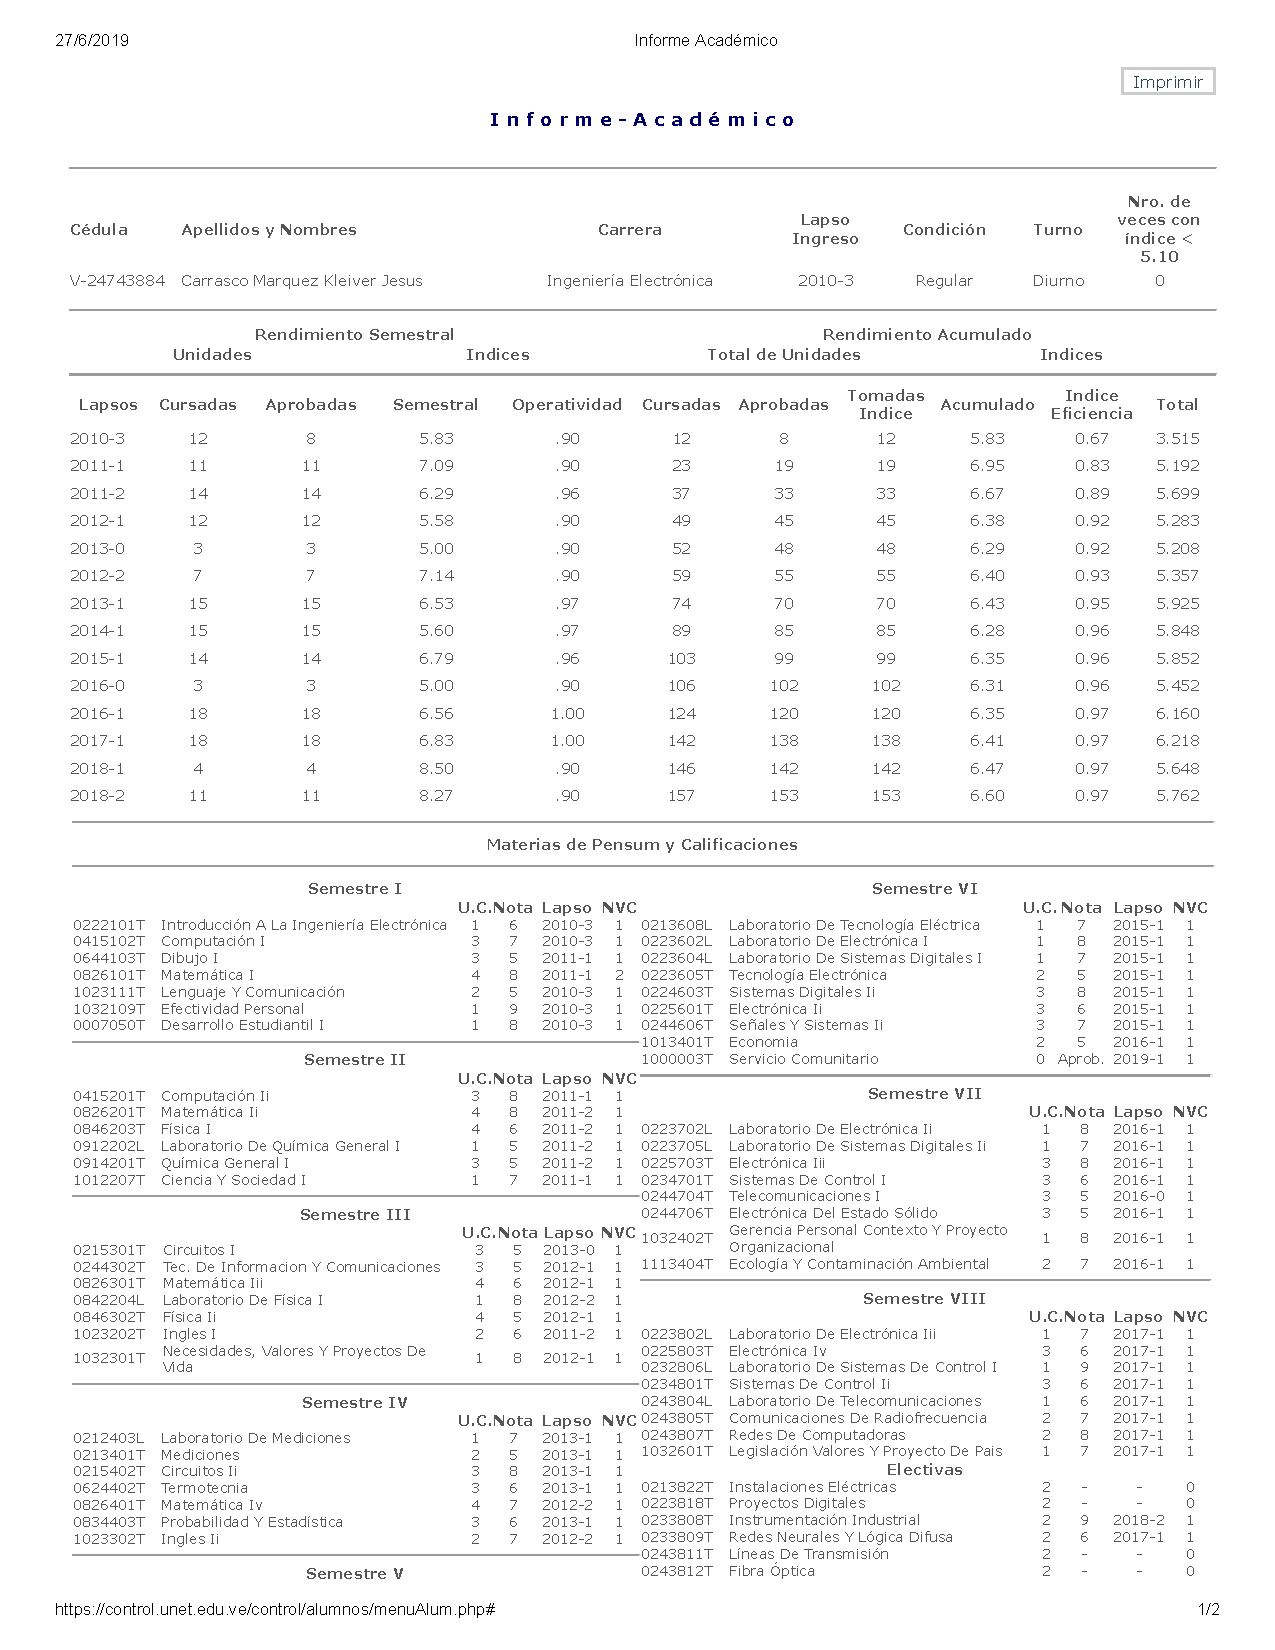
\includepdf[scale=0.7,pages=1,pagecommand={\AgregarAnexo{Informe académico}}, 
% addtotoc={1, chapter, 0,\bfseries\uppercase{Anexos}, pdf:informe}]{imagenes/informeAcademico}
% \includepdf[scale=0.7,pages=2, pagecommand={}]{imagenes/informeAcademico}
% --------------------------------------------------------------------
% Nota: Si se utiliza este código se deben comentar:
% \newpage
% \phantomsection
% \addcontentsline{toc}{chapter}{Anexos}
% --------------------------------------------------------------------

\newpage                                % Comentar si se incluye
\phantomsection                         % primero un pdf
\addcontentsline{toc}{chapter}{Anexos}  % Para evitar problemas TOC

% Para agregar anexos a la tesis
\AgregarAnexo{Interfaz grafica de la funcion de analisis de sistemas de control}{anexo:interfazAnalisis}
    \begin{figure}[htb]
        \centering
        \begin{subfigure}[t]{\textwidth}
            \centering
            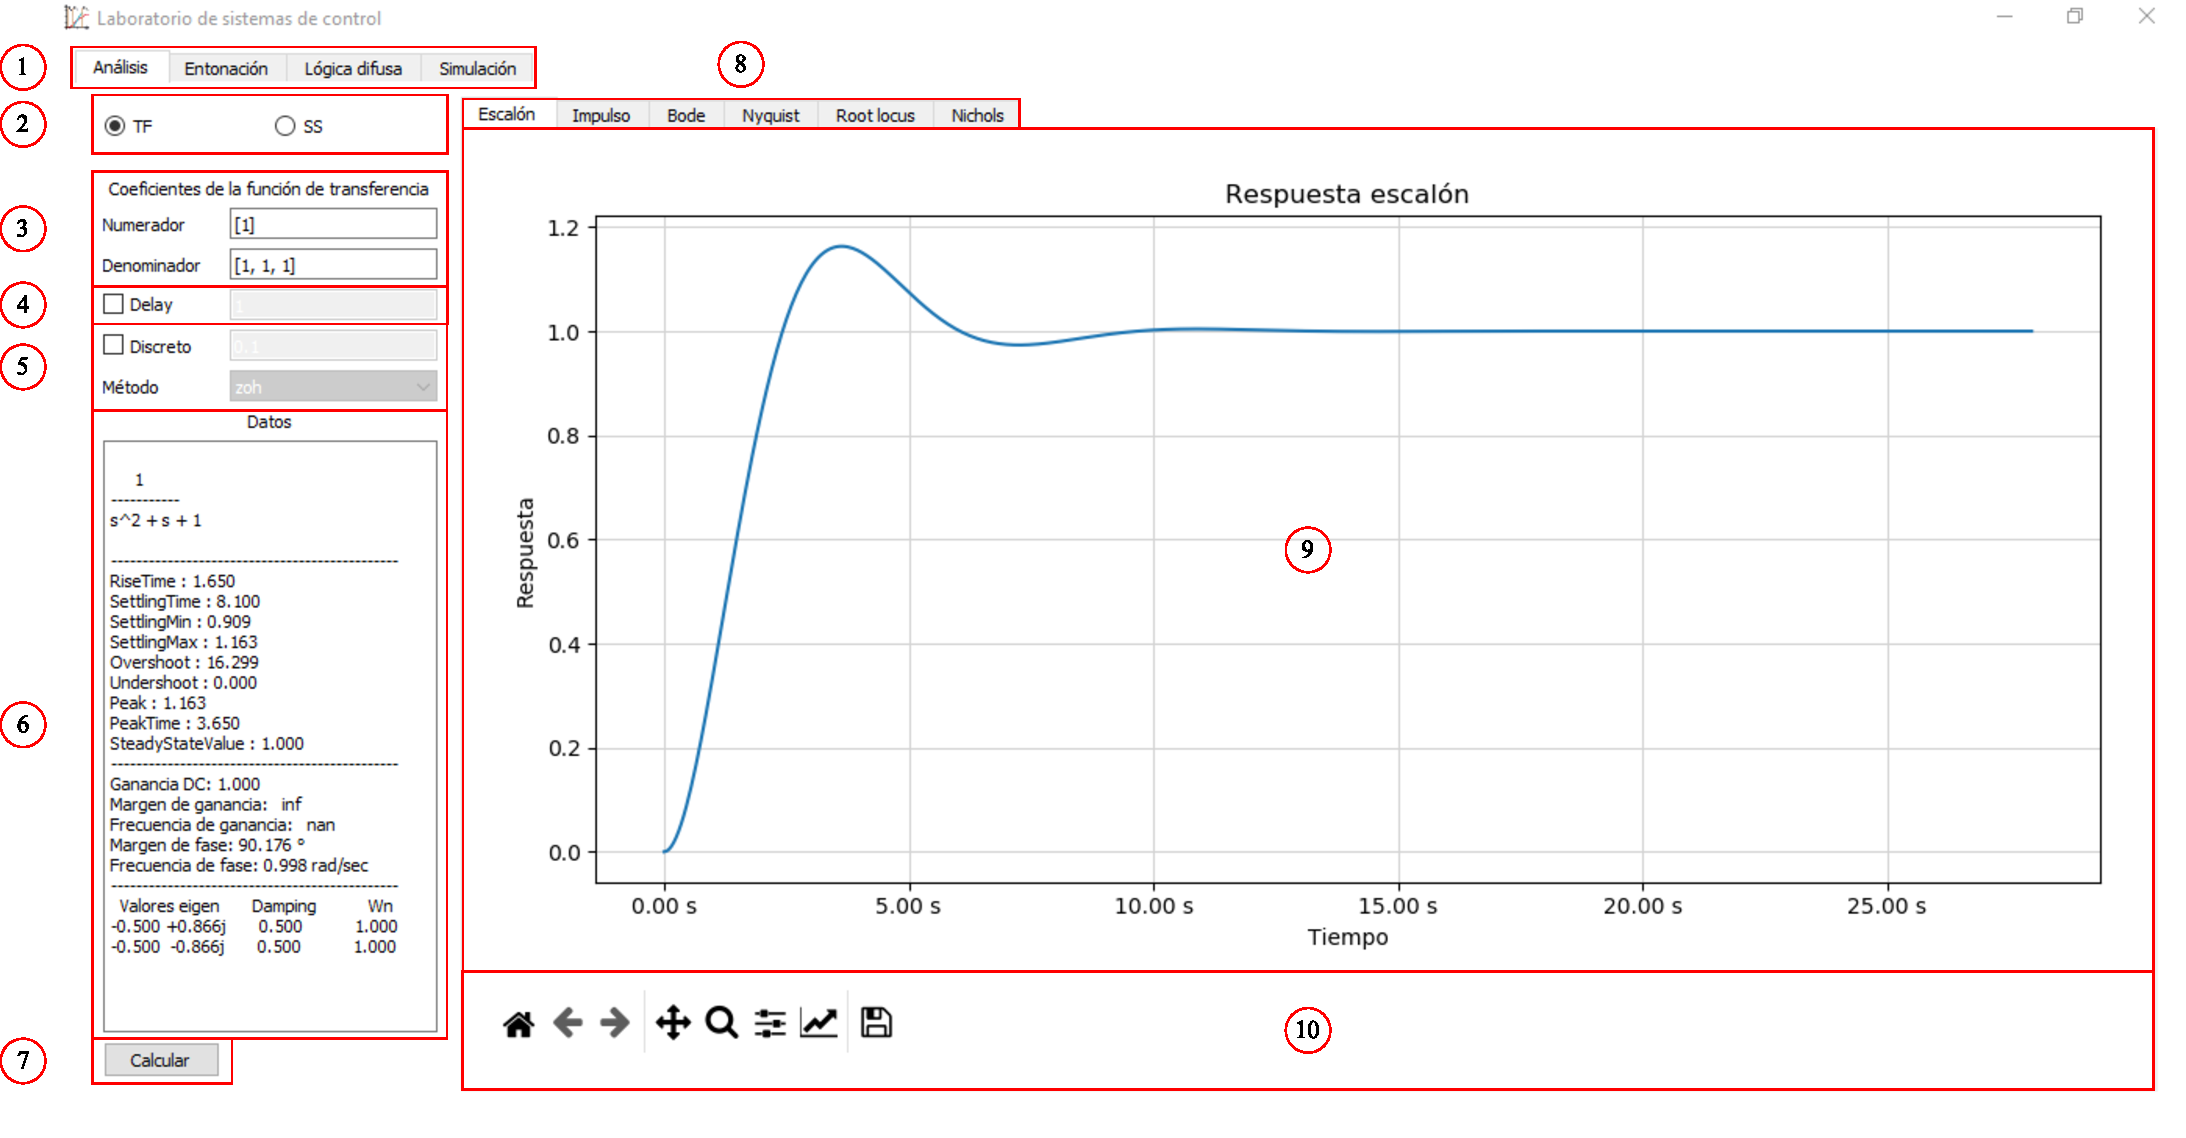
\includegraphics[width=\textwidth]{analisis.pdf}
            \caption{}
            \label{fig:interfazAnalisistf}
        \end{subfigure}
        \hfill
        \begin{subfigure}[t]{0.25\textwidth}
            \centering
            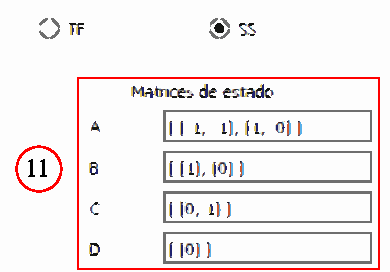
\includegraphics[width=\textwidth]{analisisSS.pdf}
            \caption{}
            \label{fig:interfazAnalisisSS}
        \end{subfigure}
        \caption[Interfaz grafica para el analisis de sistemas de control]{\textbf{Interfaz grafica para el analisis de sistemas de control}. (a) Interfaz grafica general representando al sistema con funcion de transferencia, (b) Cambios presentes si utiliza la representacion con ecuaciones de espacio de estados. Fuente: Elaboración propia. \label{fig:interfazAnalisis}}
    \end{figure}
    
    \begin{multicols}{2}
        \begin{enumerate}[leftmargin=20pt]
            \item Pestañas de funciones
            \item Selector de representación
            \item Coeficientes de la función de transferencia
            \item Agregado de Delay
            \item Discretizacion del proceso
            \item Datos del analisis
            \item Boton para realizar el analisis
            \item Pestañas de graficas
            \item Grafica con Matplotlib
            \item Barra de herramientas de la grafica
            \item Matrices de estados
        \end{enumerate}
    \end{multicols}


\AgregarAnexo{Interfaz grafica de la funcion de entonacion de controladores PID}{anexo:interfazentonacion}
    \begin{figure}[h!]
        \centering
        \begin{subfigure}[t]{\textwidth}
            \centering
            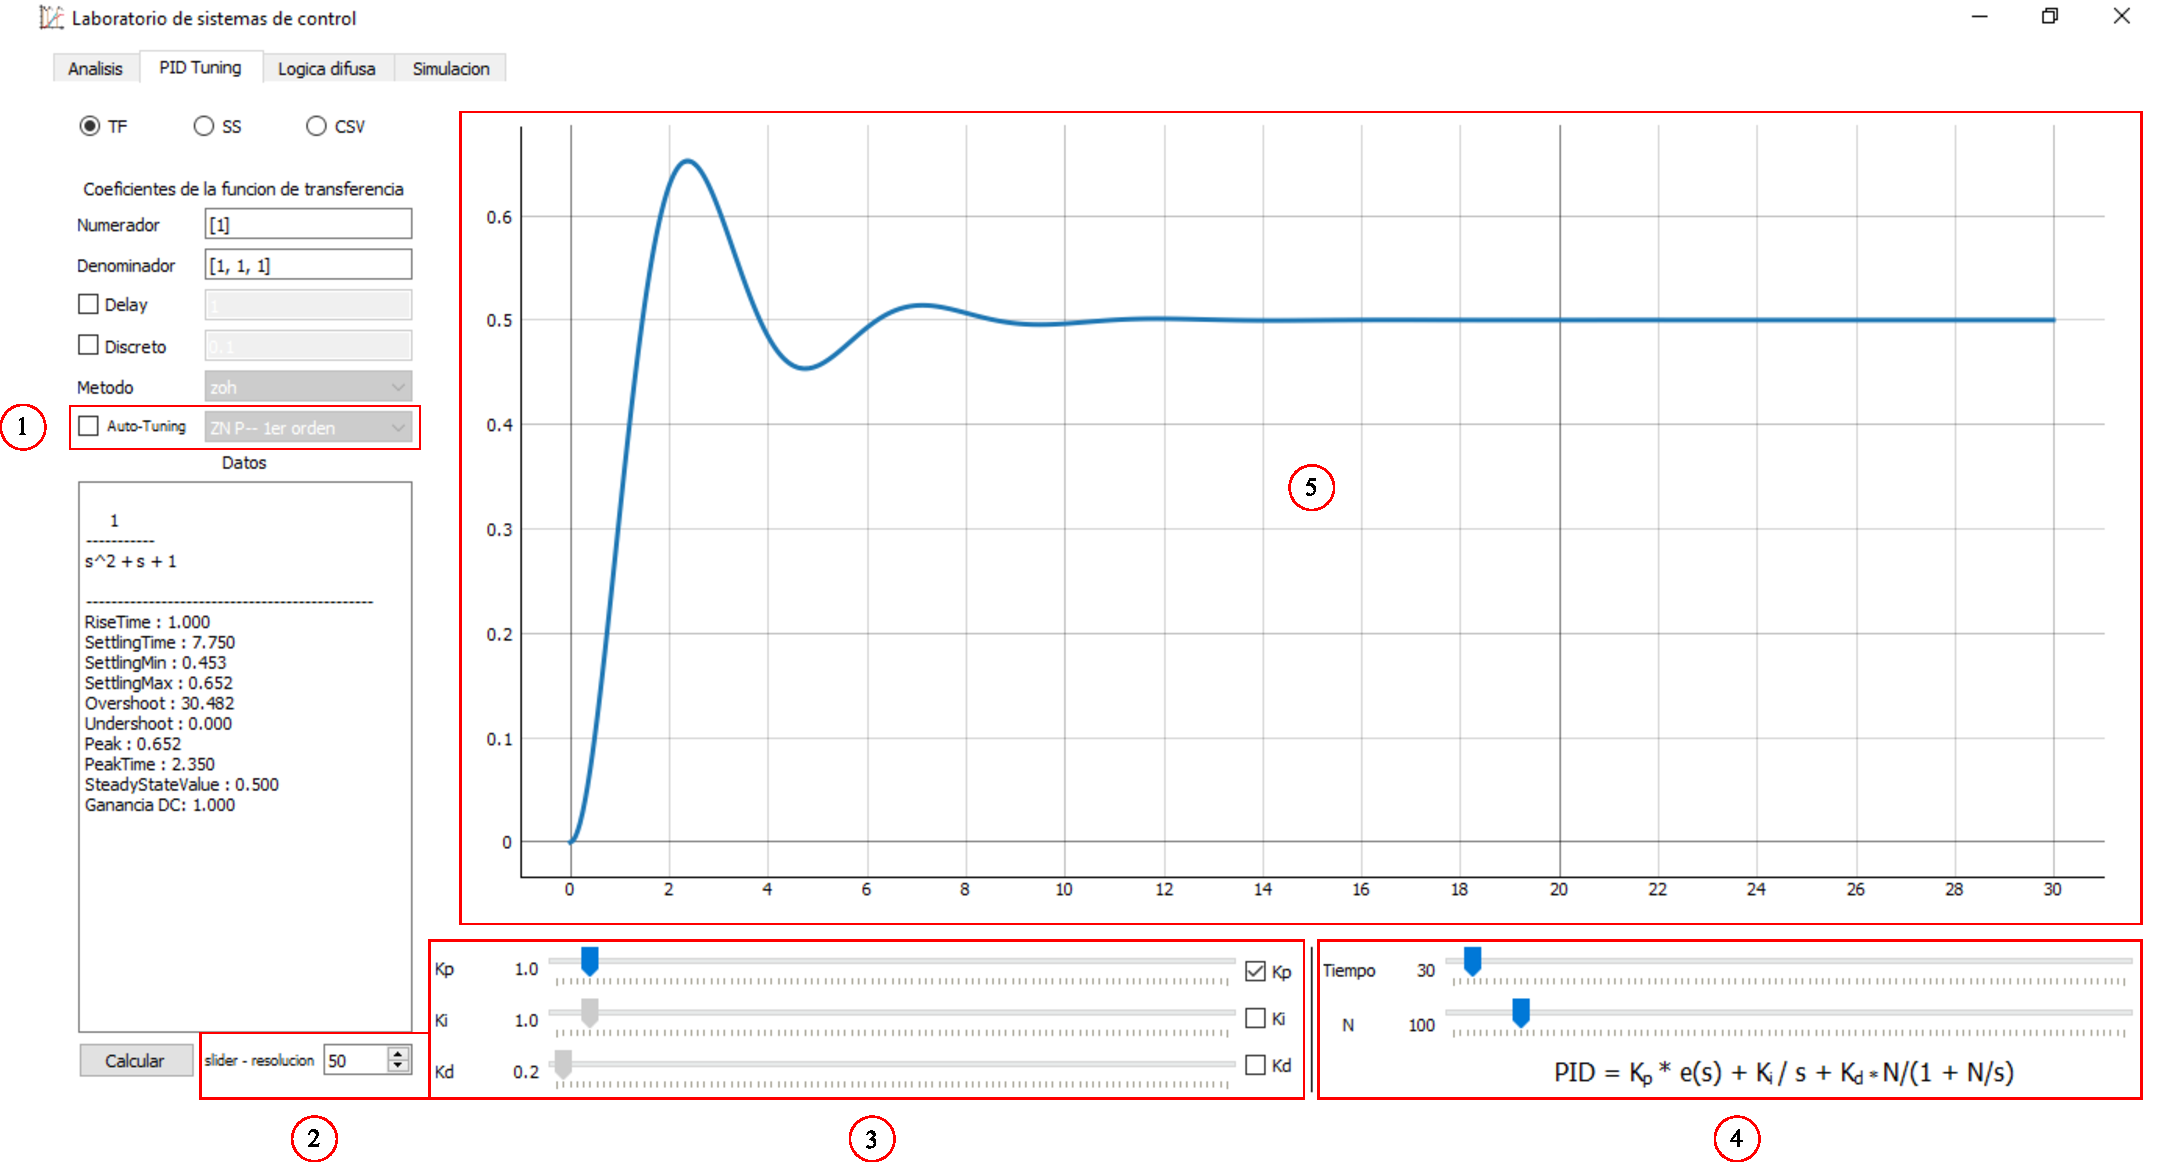
\includegraphics[width=\textwidth]{entonacionPID.pdf}
            \caption{}
            \label{fig:interfazentonacionPID}
        \end{subfigure}
        \hfill
        \begin{subfigure}[t]{\textwidth}
            \centering
            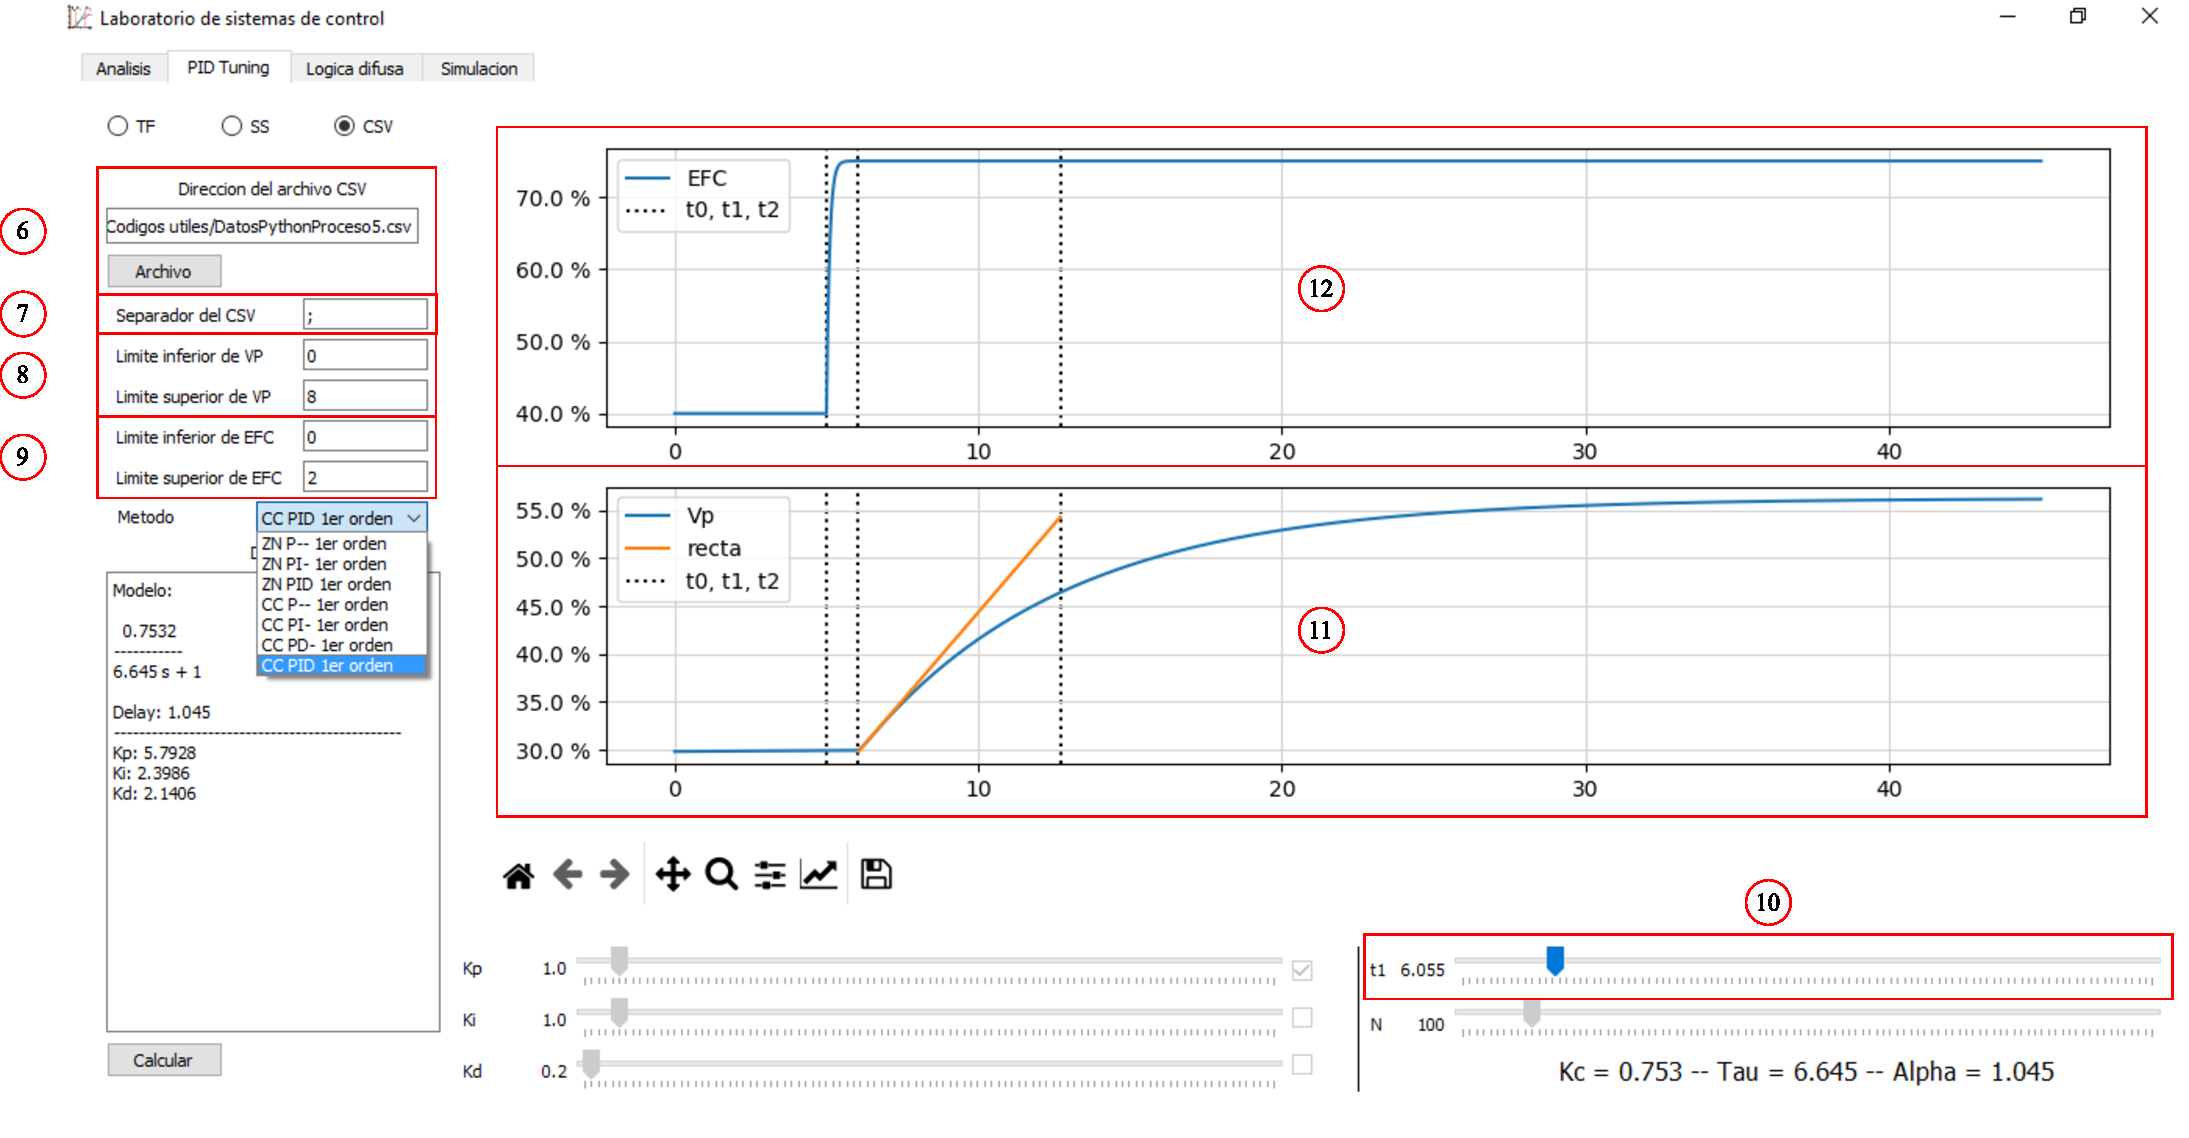
\includegraphics[width=\textwidth]{entonacionCSV.pdf}
            \caption{}
            \label{fig:interfazentonacionCSV}
        \end{subfigure}
        \caption[Interfaz grafica para el analisis de sistemas de control]{\textbf{Interfaz grafica para el analisis de sistemas de control}. (a) Interfaz grafica general para la entonación de controladores PID, (b) Interfaz grafica para la entonación utilizando un archivo CSV. Fuente: Elaboración propia. \label{fig:interfazentonacion}}
    \end{figure}
    
    \begin{multicols}{2}
        \begin{enumerate}[leftmargin=20pt]
            \item Función de entonación automática
            \item Resolución de los sliders
            \item Sliders de ganancias
            \item Sliders de tiempo y coeficiente N
            \item Gráfica con PyQtGraph
            \item Carga del archivo CSV
            \item Separador del archivo CSV
            \item SPAN de la variable del proceso
            \item SPAN de la entrada al proceso (EFC)
            \item Slider para ajustar $t_1$
            \item Gráfica de la variable del proceso
            \item Gráfica de la entrad al proceso (EFC)
        \end{enumerate}
    \end{multicols}


\AgregarAnexo{Codigo de los margenes de ganancia y fase}{anexo:margenes}
    \begin{longlisting}
        \caption[Calculo de los margenes de ganancia y fase]{Función para el calculo de los margenes de ganancia y fase.}
        \label{code:anexoA}				
        \begin{minted}[escapeinside=||,
            mathescape=true,
            autogobble=true,
            fontsize=\footnotesize,
            obeytabs=true,
            tabsize=4,
            baselinestretch=1,
			breaklines]{python}
            def margenes_ganancias(self, system, mag, phase, omega):
                """
                [Funcion para obtener el margen de ganancia y el margen de fase]
                
                :param system: [Representación del sistema]
                :type system: [LTI]
                :param mag: [Magnitud de la respuesta en frecuencia]
                :type mag: [numpyArray]
                :param phase: [Fase de la respuesta en frecuencia]
                :type phase: [numpyArray]
                :param omega: [Frecuencias utilizadas para la respuesta en frecuencia]
                :type omega: [numpyArray]
                """

                gainDb = 20 * np.log10(mag)
                degPhase = phase * 180.0 / np.pi

                # Llevando la fase a : -360 < phase < 360, para +/- 360  phase -> 0
                comp_phase = np.copy(degPhase)
                degPhase = degPhase - (degPhase/360).astype(int) * 360

                # Para evitar la deteccion de cruces al llevar las fases al rango -360 < phase < 360
                crossHack1 = np.diff(1 * (degPhase > -183) != 0)
                crossHack2 = np.diff(1 * (degPhase > -177) != 0)
                crossHack = ~crossHack1 * ~crossHack2

                # Deteccion de cruce
                indPhase = np.diff(1 * (gainDb > 0) != 0)
                indGain = np.diff(1 * (degPhase > -180) != 0)
                indGain = indGain * crossHack

                # Calculo de la respuesta en frecuencia para omega = 0 rad/s
                zero_freq_response = ctrl.evalfr(system, 0j)
                omega = np.insert(omega, 0, 0)
                zeroPhase = np.angle(zero_freq_response)
                zeroMag = np.abs(zero_freq_response)
                if zeroPhase * 180.0 / np.pi >= 180:
                    zeroPhase = zeroPhase - 2 * np.pi
                gainDb = np.insert(gainDb, 0, 20 * np.log10(zeroMag))
                degPhase = np.insert(degPhase, 0, zeroPhase * 180.0 / np.pi)

                # Verificando "cruce" por -180 grados para omega = 0 rad/s
                if zeroPhase * 180.0 / np.pi == -180:
                    indGain = np.insert(indGain, 0, True)
                else:
                    indGain = np.insert(indGain, 0, False)

                # Verificando "cruce" por 0 dB para omega = 0 rad/s
                if 20 * np.log10(zeroMag) == 0:
                    indPhase = np.insert(indPhase, 0, True)
                else:
                    indPhase = np.insert(indPhase, 0, False)

                # Margen de ganancia
                if len(omega[:-1][indGain]) > 0:
                    newGainIndex = np.argmin(np.abs(gainDb[:-1][indGain]))
                    omegaGain = omega[:-1][indGain][newGainIndex]
                    GainMargin = -gainDb[:-1][indGain][newGainIndex]
                else:
                    omegaGain = np.nan
                    GainMargin = np.infty

                # Margen de Fase
                if len(omega[:-1][indPhase]) > 0:
                    newPhaIndex = min(range(len(degPhase[:-1][indPhase])),
                                    key=lambda i: abs(np.abs(degPhase[:-1][indPhase][i]) - 180))
                    omegaPhase = omega[:-1][indPhase][newPhaIndex]
                    PhaseMargin = 180 + degPhase[:-1][indPhase][newPhaIndex]
                else:
                    omegaPhase = np.nan
                    PhaseMargin = np.infty

                return GainMargin, PhaseMargin, omegaGain, omegaPhase
        \end{minted}
    \end{longlisting}

\AgregarAnexo{Ejemplo de un archivo CSV valido para la entonacion}{anexo:csv}
    \begin{longlisting}				
        \begin{minted}[escapeinside=||,
            mathescape=true,
            autogobble=true,
            fontsize=\footnotesize,
            obeytabs=true,
            tabsize=4,
            baselinestretch=1,
            breaklines]{text}
            $Date;$Time;VP2;EFC2;SP2
            02/22/12;01:21:00.000;0.6312256;5.233645;1.009346
            02/22/12;01:21:00.070;0.6312256;5.233645;1.009346
            02/22/12;01:21:00.140;0.6312256;5.233645;1.009346
            02/22/12;01:21:00.210;0.6312256;5.233645;1.009346
            02/22/12;01:21:00.280;0.6312256;5.233645;1.009346
            02/22/12;01:21:00.350;0.6312256;5.233645;1.009346
            02/22/12;01:21:00.420;0.6312256;5.233645;1.009346
            02/22/12;01:21:00.490;0.6312256;5.233645;1.009346
            02/22/12;01:21:00.560;0.6312256;5.233645;1.009346
            02/22/12;01:21:00.630;0.6312256;5.233645;1.009346
            02/22/12;01:21:00.700;0.6312256;5.233645;1.009346
            02/22/12;01:21:00.770;0.6312256;5.233645;1.009346
            02/22/12;01:21:00.840;0.6313477;5.233645;1.009346
            02/22/12;01:21:00.910;0.6313477;5.233645;1.009346
            02/22/12;01:21:00.980;0.6313477;5.233645;1.009346
            02/22/12;01:21:01.050;0.6313477;5.233645;1.009346
            02/22/12;01:21:01.120;0.6313477;5.233645;1.009346
            02/22/12;01:21:01.190;0.6313477;5.233645;1.009346
            02/22/12;01:21:01.260;0.6313477;5.233645;1.009346
            02/22/12;01:21:01.330;0.6313477;5.233645;1.009346
            02/22/12;01:21:01.400;0.6313477;5.233645;1.009346
            02/22/12;01:21:01.470;0.6313477;5.233645;1.009346
            |$\qquad\vdots\qquad\qquad\qquad\vdots\quad\qquad\qquad\vdots\qquad\qquad\quad\vdots\qquad\qquad\vdots$|
            02/22/12;01:21:34.300;1.676147;6.654205;1.009346
            02/22/12;01:21:34.370;1.676147;6.654205;1.009346
            02/22/12;01:21:34.440;1.676147;6.654205;1.009346
            02/22/12;01:21:34.510;1.676147;6.654205;1.009346
            02/22/12;01:21:34.580;1.676147;6.654205;1.009346
            02/22/12;01:21:34.650;1.676147;6.654205;1.009346
            02/22/12;01:21:34.720;1.676147;6.654205;1.009346
            02/22/12;01:21:34.790;1.675903;6.654205;1.009346
            02/22/12;01:21:34.860;1.675903;6.654205;1.009346
            02/22/12;01:21:34.930;1.675903;6.654205;1.009346
            02/22/12;01:21:35.000;1.675903;6.654205;1.009346
        \end{minted}
    \end{longlisting}

    Esta data es valida porque posee tres o mas columnas, de las cuales, tres poseen un encabezado con las palabras claves necesarias (VP, EFC y TIME), se esta utilizando un separador valido (;), el formato de tiempo es correcto (hh:mm:ss) y la respuesta de la variable del proceso es ascendente.

 \AgregarAnexo{Codigo de transformacion equivalente entre funciones de membresia}{anexo:mfequivalencia}
    \begin{longlisting}
        \caption[Transformación equivalente entre funciones de membresía]{Función para la transformación equivalente entre funciones de membresía.}
        \label{code:anexoC}				
        \begin{minted}[escapeinside=||,
            mathescape=true,
            autogobble=true,
            fontsize=\footnotesize,
            obeytabs=true,
            tabsize=4,
            baselinestretch=1,
			breaklines]{python}
            def update_definicionmf(self, old_mf, definicion, new_mf):
                """
                [Funcion para la transformacion equivalente entre funciones de membresia]
                
                :param old_mf: [Nombre de la antigua funcion de membresia]
                :type old_mf: [str]
                :param definicion: [Lista con los valroes correspondiente a la definicion de la antigua funcion de membresia]
                :type definicion: [list]
                :param new_mf: [Nombre de la nueva funcion de membresia]
                :type new_mf: [str]
                """
                
                if old_mf == 'trimf':
                    a, b, c = definicion

                    if new_mf == 'trimf':
                        na, nb, nc = a, b, c
                        return [na, nb, nc], '[a, b, c] con: a <= b <= c'

                    if new_mf == 'trapmf':
                        na, nd = a, c
                        nb = (a+b) / 2
                        nc = (b+c) / 2
                        return [na, nb, nc, nd], '[a, b, c, d] con: a <= b <= c <= d'

                    if new_mf == 'gaussmf':
                        mean = b
                        sigma = (abs(c) + abs(a)) / 8
                        return [sigma, mean], '[sigma, media]'

                    if new_mf == 'gauss2mf':
                        mean1 = (a+b) / 2
                        sigma1 = (abs(c) + abs(a)) / 16
                        mean2 = (b+c) / 2
                        sigma2 = (abs(c) + abs(a)) / 16
                        return [sigma1, mean1, sigma2, mean2], '[sigma1, media1, sigma2, media2] con: media1 <= media2'

                    if new_mf == 'smf' or new_mf == 'zmf':
                        na = (a+b) / 2
                        nb = (b+c) / 2
                        return [na, nb], '[a, b] siendo a el inicio del cambio \ny b el final del cambio'

                    if new_mf == 'sigmf':
                        nb = b
                        nc = 10 / (abs(c) + abs(a))
                        return [nc, nb], '[a, b] con:\n a como el ancho del sigmoide, puede ser negativo\n b el centro del sigmoide'

                    if new_mf == 'dsigmf':
                        nb1 = (a+b) / 2
                        nc1 = 20 / (abs(c) + abs(a))
                        nb2 = (b+c) / 2
                        nc2 = -20 / (abs(c) + abs(a))
                        return [nc1, nb1, nc2, nb2], '[a1, b1, a2, b2] con:\n b1, b2 como los centros de los sigmoides\n a1, a2 los anchos de los sigmoides, pueden ser negativos'

                    if new_mf == 'psigmf':
                        nb1 = (a+b) / 2
                        nc1 = 20 / (abs(c) + abs(a))
                        nb2 = (b+c) / 2
                        nc2 = -20 / (abs(c) + abs(a))
                        return [nc1, nb1, nc2, nb2], '[a1, b1, a2, b2] con:\n b1, b2 como los centros de los sigmoides\n a1, a2 los anchos de los sigmoides, pueden ser negativos'

                    if new_mf == 'pimf':
                        na, nd = a, c
                        nb = (a+b) / 2
                        nc = (b+c) / 2
                        return [na, nb, nc, nd], '[a, b, c, d] con:\na inicio de la subida y b su final por el lado izquierdo \nc inicio de la bajada y d su final por el lado derecho'

                    if new_mf == 'gbellmf':
                        na = abs(c) - abs(a)
                        nb = 1 / (a-b)
                        nc = b
                        return [na, nb, nc], '[a, b, c] con:\na como el ancho de la camapana\nb pendiente de la campana, puede ser negativa\nc centro de la camapana'

                if old_mf == 'trapmf':
                    a, b, c, d = definicion
                    na, nc = a, d
                    nb = (c+b) / 2
                    return [na, nb, nc], '[a, b, c] con: a <= b <= c'

                if old_mf == 'gaussmf':
                    b, a = definicion
                    na = a - b*4
                    nc = a + b*4
                    nb = a
                    return [na, nb, nc], '[a, b, c] con: a <= b <= c'

                if old_mf == 'gauss2mf':
                    b, a, d, c = definicion
                    na = a - b*4
                    nc = c + d*4
                    nb = (a+c) / 2
                    return [na, nb, nc], '[a, b, c] con: a <= b <= c'

                if old_mf == 'smf' or old_mf == 'zmf':
                    a, c = definicion
                    na = a - (abs(a) + abs(c)) / 4
                    nc = c + (abs(a) + abs(c)) / 4
                    nb = (a+c) / 2
                    return [na, nb, nc], '[a, b, c] con: a <= b <= c'

                if old_mf == 'sigmf':
                    c, b = definicion
                    na = b - abs(c) * 5
                    nb = b
                    nc = b + abs(c) * 5
                    return [na, nb, nc], '[a, b, c] con: a <= b <= c'

                if old_mf == 'dsigmf':
                    b, a, d, c = definicion
                    na = a - b*1.25
                    nb = (a+c) / 2
                    nc = c - d*1.25
                    return [na, nb, nc], '[a, b, c] con: a <= b <= c'

                if old_mf == 'psigmf':
                    b, a, d, c = definicion
                    na = a - b*1.25
                    nb = (a+c) / 2
                    nc = c - d*1.25
                    return [na, nb, nc], '[a, b, c] con: a <= b <= c'

                if old_mf == 'pimf':
                    a, b, c, d = definicion
                    na, nc = a, d
                    nb = (c+b) / 2
                    return [na, nb, nc], '[a, b, c] con: a <= b <= c'

                if old_mf == 'gbellmf':
                    a, b, c = definicion
                    na = c - abs(a / c)
                    nb = c
                    nc = c + abs(a / c)
                    return [na, nb, nc], '[a, b, c] con: a <= b <= c'
        \end{minted}
    \end{longlisting}

\AgregarAnexo{Esquemas de control difuso}{anexo:esquemas}
    
    \vfill

    \begin{figure}[htb]
        \centering
        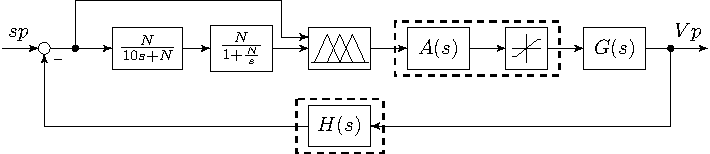
\includegraphics[width=\textwidth]{pdDifuso.pdf}
        \caption[Esquema de control implementado: PD difuso]{\textbf{Esquema de control implementado: PD difuso}. Fuente: Elaboración propia.} 
        \label{fig:pdDifuso}
    \end{figure}
    
    \vfill

    \begin{figure}[htb]
        \centering
        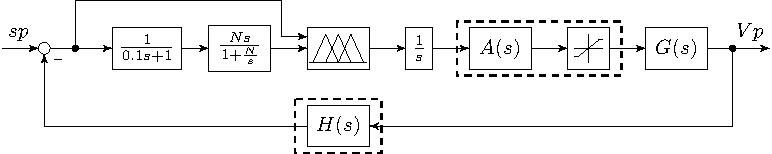
\includegraphics[width=\textwidth]{piDifuso.pdf}
        \caption[Esquema de control implementado: PI difuso]{\textbf{Esquema de control implementado: PI difuso}. Fuente: Elaboración propia.} 
        \label{fig:piDifuso}
    \end{figure}

    \vfill

    \begin{figure}[htb]
        \centering
        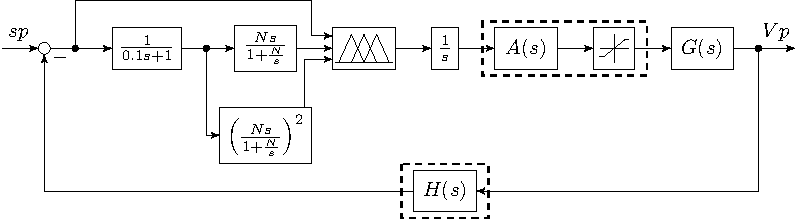
\includegraphics[width=\textwidth]{pidDifuso.pdf}
        \caption[Esquema de control implementado: PID difuso]{\textbf{Esquema de control implementado: PID difuso}. Fuente: Elaboración propia.} 
        \label{fig:pidDifuso}
    \end{figure}
    
    \vfill

    \pagebreak
    
    \vfill

    \begin{figure}[htb]
        \centering
        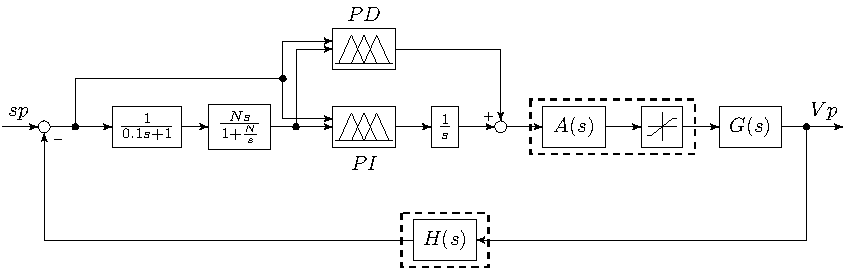
\includegraphics[width=\textwidth]{pipdDifuso.pdf}
        \caption[Esquema de control implementado: PD difuos mas PI difuso]{\textbf{Esquema de control implementado: PD difuos mas PI difuso}. Fuente: Elaboración propia.} 
        \label{fig:pipdDifuso}
    \end{figure}
    
    \vfill

    \begin{figure}[htb]
        \centering
        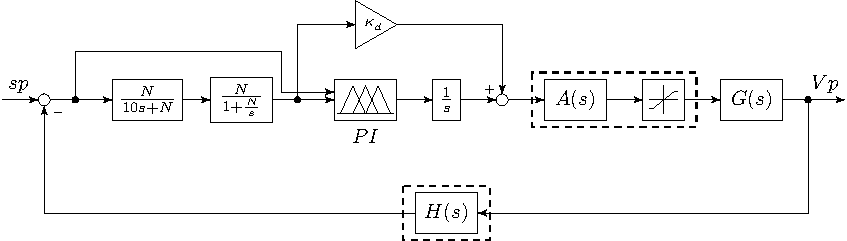
\includegraphics[width=\textwidth]{piplusDDifuso.pdf}
        \caption[Esquema de control implementado: PI difuso mas derivada]{\textbf{Esquema de control implementado: PI difuso mas derivada}. Fuente: Elaboración propia.} 
        \label{fig:piplusDDifuso}
    \end{figure}
    
    \vfill

    \begin{figure}[htb]
        \centering
        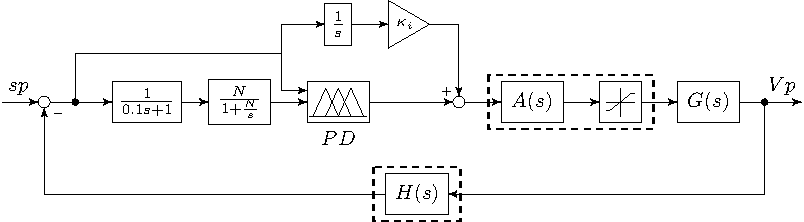
\includegraphics[width=\textwidth]{pdplusIDifuso.pdf}
        \caption[Esquema de control implementado: PD difuso mas integrador]{\textbf{Esquema de control implementado: PD difuso mas integrador}. Fuente: Elaboración propia.} 
        \label{fig:pdplusIDifuso}
    \end{figure}
    
    \vfill

    \pagebreak
    
    \vfill

    \begin{figure}[htb]
        \centering
        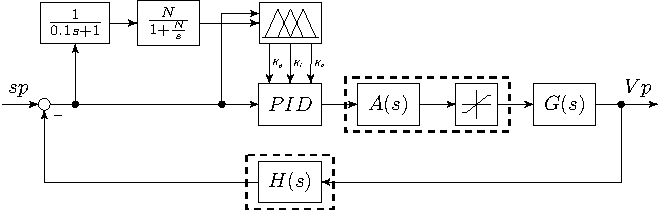
\includegraphics[width=\textwidth]{GainScheduler.pdf}
        \caption[Esquema de control implementado: Programador de ganancias]{\textbf{Esquema de control implementado: Programador de ganancias}. Fuente: Elaboración propia.} 
        \label{fig:GainScheduler}
    \end{figure}
    
    \vfill

    \begin{figure}[htb]
        \centering
        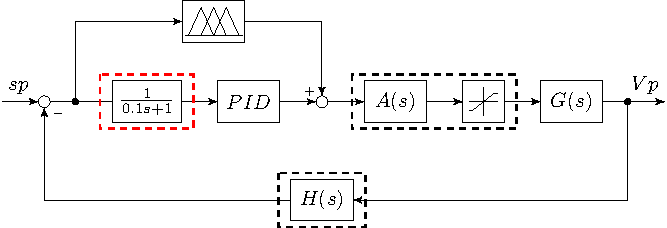
\includegraphics[width=\textwidth]{pidplusDifuso.pdf}
        \caption[Esquema de control implementado: PID clasico mas P difuso]{\textbf{Esquema de control implementado: PID clasico mas P difuso}. Fuente: Elaboración propia.} 
        \label{fig:pidplusDifuso}
    \end{figure}
    
    \vfill

\AgregarAnexo{Formato interno para guardar controlador por medio de un archivo .JSON}{anexo:json}
    \begin{longlisting}
        \caption[Formato para guardar controlador]{Formato para un controlador con una entrada, una salida y tres reglas. Las reglas son: una simple, una regla con premisa negada y una regla con salida ponderada en 0.25.}
        \label{code:anexoE}				
        \begin{minted}[escapeinside=||,
            mathescape=true,
            autogobble=true,
            fontsize=\footnotesize,
            obeytabs=true,
            tabsize=4,
            baselinestretch=1,
			breaklines]{python}
            [
                [
                    {
                        "nombre": "entrada1",
                        "numeroE": 3,
                        "etiquetas": [
                            {
                                "nombre": "etiqueta1",
                                "mf": "trimf",
                                "definicion": [
                                    -20.0,
                                    -10.0,
                                    0.0
                                ]
                            },
                            {
                                "nombre": "etiqueta2",
                                "mf": "trapmf",
                                "definicion": [
                                    -10.0,
                                    -5.0,
                                    5.0,
                                    10.0
                                ]
                            },
                            {
                                "nombre": "etiqueta3",
                                "mf": "gaussmf",
                                "definicion": [
                                    2.5,
                                    10.0
                                ]
                            }
                        ],
                        "rango": [
                            -10,
                            10
                        ]
                    }
                ],
                [
                    {
                        "nombre": "salida1",
                        "numeroE": 3,
                        "etiquetas": [
                            {
                                "nombre": "etiqueta1",
                                "mf": "gauss2mf",
                                "definicion": [
                                    1.25,
                                    -15.0,
                                    1.25,
                                    -5.0
                                ]
                            },
                            {
                                "nombre": "etiqueta2",
                                "mf": "dsigmf",
                                "definicion": [
                                    1.0,
                                    -5.0,
                                    1.0,
                                    5.0
                                ]
                            },
                            {
                                "nombre": "etiqueta3",
                                "mf": "pimf",
                                "definicion": [
                                    0.0,
                                    5.0,
                                    15.0,
                                    20.0
                                ]
                            }
                        ],
                        "rango": [
                            -10,
                            10
                        ],
                        "metodo": "centroid"
                    }
                ],
                [
                    [
                        [
                            [
                                "etiqueta1",
                                0,
                                false
                            ]
                        ],
                        [
                            [
                                "etiqueta1",
                                0,
                                1.0
                            ]
                        ],
                        true
                    ],
                    [
                        [
                            [
                                "etiqueta2",
                                0,
                                true
                            ]
                        ],
                        [
                            [
                                "etiqueta2",
                                0,
                                1.0
                            ]
                        ],
                        false
                    ],
                    [
                        [
                            [
                                "etiqueta3",
                                0,
                                false
                            ]
                        ],
                        [
                            [
                                "etiqueta3",
                                0,
                                0.24999999999999933
                            ]
                        ],
                        false
                    ]
                ]
            ]
        \end{minted}
    \end{longlisting}

\AgregarAnexo{Codigos para el manejo de archivos FIS}{anexo:codefis}
    \begin{longlisting}
        \caption[Extraccion de datos del archivo FIS - YAPFLM]{Extraccion de datos del archivo FIS - YAPFLM.}
        \label{code:anexoF1}				
        \begin{minted}[escapeinside=||,
            mathescape=true,
            autogobble=true,
            fontsize=\footnotesize,
            obeytabs=true,
            tabsize=4,
            baselinestretch=1,
			breaklines]{python}
            class FISParser:
                """
                [Clase para cargar y exportar archivos .fis, para cargar los archivos FIS las funciones get_system, get_vars, get_var y get_rules fueron tomadas de yapflm (Yet Another Python Fuzzy Logic Module) para obtener los datos necesarias del .fis, de alli, se aplica la funcion fis_to_json para completar el parsin.
                
                En el caso de la exportancion, se realiza utilizando la funcion json_to_fis]
                """

                def __init__(self, file, InputList=None, OutputList=None, RuleEtiquetas=None):
                    """
                    [Constructor de la clase, inicializa las variables a utilizar y selecciona entre cargar el fis o exportarlo dependiendo de las variables con las que se cree el objeto]
                    
                    :param file: [Direccion del archivo a cargar o exportar]
                    :type file: [str]
                    :param inputlist: [Lista de variables de entrada], defaults to None
                    :type inputlist: [list], optional
                    :param OutputList: [Lista de variables de entrada], defaults to None
                    :type OutputList: [list], optional
                    :param RuleEtiquetas: [Lista con la informacion necesaria para crear las reglas], defaults to None
                    :type RuleEtiquetas: [list], optional
                    """

                    # Cargar archivo .fis
                    if InputList is None and OutputList is None and RuleEtiquetas is None:
                        with open(file, 'r') as infis:
                            self.rawlines = infis.readlines()
                        self.systemList = 0
                        self.InputList = []
                        self.OutputList = []
                        self.RuleList = []
                        self.get_system()
                        self.get_vars()
                        self.get_rules()
                    else:
                        # Exportar archivo .fis
                        self.file = file
                        self.InputList = InputList
                        self.OutputList = OutputList
                        self.RuleEtiquetas = RuleEtiquetas
                        self.json_to_fis()

                def get_system(self):
                    """ [Funcion tomada de yapflm (Yet Another Python Fuzzy Logic Module)] """
                    
                    end_sysblock = self.rawlines.index('\n')
                    systemblock = self.rawlines[1:end_sysblock]
                    fisargs = map(lambda x: parse('{arg}={val}', x), systemblock)
                    fissys = {f['arg'].lower(): f['val'].strip("'") for f in fisargs}
                    self.numinputs = int(fissys['numinputs'])
                    self.numoutputs = int(fissys['numoutputs'])
                    self.numrules = int(fissys['numrules'])
                    self.start_varblocks = end_sysblock + 1
                    self.systemList = fissys

                def get_var(self, vartype, varnum, start_line, end_line):
                    """ [Funcion tomada de yapflm (Yet Another Python Fuzzy Logic Module)] """
                    
                    varblock = self.rawlines[start_line:end_line]
                    fisargs = map(lambda x: parse('{arg}={val}', x), varblock)
                    fisvar = {f['arg'].lower(): f['val'].strip("'") for f in fisargs}

                    if 'input' in vartype:
                        self.InputList.append(fisvar)
                    elif 'output' in vartype:
                        self.OutputList.append(fisvar)

                def get_vars(self):
                    """ [Funcion tomada de yapflm (Yet Another Python Fuzzy Logic Module)] """
                    
                    start_ruleblock = self.rawlines.index('[Rules]\n')
                    var_lines = []
                    var_types = []
                    flag = 0
                    for i, line in enumerate(self.rawlines[self.start_varblocks - 1:start_ruleblock]):
                        if flag:
                            flag = 0
                            vt = parse('[{type}{num:d}]', line)
                            var_types.append((vt['type'].lower(), vt['num']))
                        if line == '\n':
                            var_lines.append(i + self.start_varblocks - 1)
                            flag = 1
                    for i, l in enumerate(var_lines[:-1]):
                        if 'input' in var_types[i][0]:
                            self.get_var('input', var_types[i][1] - 1, l + 2, var_lines[i + 1])
                        elif 'output' in var_types[i][0]:
                            self.get_var('output', var_types[i][1] - 1, l + 2, var_lines[i + 1])

                def get_rules(self):
                    """ [Funcion tomada de yapflm (Yet Another Python Fuzzy Logic Module)] """
                    
                    start_ruleblock = self.rawlines.index('[Rules]\n')
                    ruleblock = self.rawlines[start_ruleblock + 1:]
                    antecedents = (('{a%d:d} ' * self.numinputs) %
                                tuple(range(self.numinputs))).strip()
                    consequents = ('{c%d:d} ' * self.numoutputs) % tuple(range(self.numoutputs))
                    p = antecedents + ', ' + consequents + '({w:d}) : {c:d}'
                    for rule in ruleblock:
                        try:
                            p = antecedents + ', ' + consequents + '({w:d}) : {c:d}'
                            rp = parse(p, rule)
                            r = []
                            for inp in range(self.numinputs):
                                rpar = rp['a%d' % inp]
                                rval = rpar if rpar != 0 else None
                                r.append(rval)
                            for outp in range(self.numoutputs):
                                rpar = rp['c%d' % outp]
                                rval = rpar if rpar != 0 else None
                                r.append(rval)
                            r += [rp['w'], rp['c'] - 1]
                            self.RuleList.append(r)
                        except:
                            p = antecedents + ', ' + consequents + '({w:f}) : {c:d}'
                            rp = parse(p, rule)
                            r = []
                            for inp in range(self.numinputs):
                                rpar = rp['a%d' % inp]
                                rval = rpar if rpar != 0 else None
                                r.append(rval)
                            for outp in range(self.numoutputs):
                                rpar = rp['c%d' % outp]
                                rval = rpar if rpar != 0 else None
                                r.append(rval)
                            r += [rp['w'], rp['c'] - 1]
                            self.RuleList.append(r)
        \end{minted}
    \end{longlisting}

    \begin{longlisting}
        \caption[Procesado de los datos del FIS]{Procesado de los datos del FIS, esta funcion pertenece a la clase FISParser.}
        \label{code:anexoF2}				
        \begin{minted}[escapeinside=||,
            mathescape=true,
            autogobble=true,
            fontsize=\footnotesize,
            obeytabs=true,
            tabsize=4,
            baselinestretch=1,
            breaklines]{python}
            def fis_to_json(self):
                """ [Funcion para completar la creacion del controlador a partir de un archivo .fis] """
                
                # Datos del controlador
                ni = int(self.systemList['numinputs'])
                no = int(self.systemList['numoutputs'])
                nr = int(self.systemList['numrules'])

                InputList = [0] * ni
                OutputList = [0] * no
                RuleEtiquetas = []

                # Creacion de las variables de entrada
                for i in range(ni):
                    InputList[i] = {
                        "nombre":
                            self.InputList[i]['name'],
                        "numeroE":
                            int(self.InputList[i]['nummfs']),
                        "etiquetas": [0] * int(self.InputList[i]['nummfs']),
                        "rango":
                            ast.literal_eval(
                                re.sub("\s+", ",", self.InputList[i]['range'].strip()))
                    }

                    for ne in range(int(self.InputList[i]['nummfs'])):
                        temp_etiqueta = self.InputList[0]['mf' + str(ne + 1)].replace(
                            "'", '').split(':')
                        temp2 = temp_etiqueta[1].split(',')
                        InputList[i]['etiquetas'][ne] = {
                            "nombre": temp_etiqueta[0],
                            "mf": temp2[0],
                            "definicion": ast.literal_eval(re.sub("\s+", ",", temp2[1].strip()))
                        }

                # Creacion de las variables de salida
                for i in range(no):
                    OutputList[i] = {
                        "nombre":
                            self.OutputList[i]['name'],
                        "numeroE":
                            int(self.OutputList[i]['nummfs']),
                        "etiquetas": [0] * int(self.OutputList[i]['nummfs']),
                        "rango":
                            ast.literal_eval(
                                re.sub("\s+", ",", self.OutputList[i]['range'].strip())),
                        "metodo":
                            self.systemList['defuzzmethod']
                    }

                    for ne in range(int(self.OutputList[i]['nummfs'])):
                        temp_etiqueta = self.OutputList[i]['mf' + str(ne + 1)].replace(
                            "'", '').split(':')
                        temp2 = temp_etiqueta[1].split(',')
                        OutputList[i]['etiquetas'][ne] = {
                            "nombre": temp_etiqueta[0],
                            "mf": temp2[0],
                            "definicion": ast.literal_eval(re.sub("\s+", ",", temp2[1].strip()))
                        }
                        
                # Creacion de las reglas
                for numeror, i in enumerate(self.RuleList):
                    ril = []
                    rol = []

                    for j in range(ni):
                        if i[j] is not None:
                            nombre = InputList[j]['etiquetas'][abs(i[j]) - 1]['nombre']
                            numero = j
                            negacion = False if i[j] > 0 else True
                            ril.append([nombre, numero, negacion])

                    for j in range(ni, no + ni):
                        if i[j] is not None:
                            if i[j] < 0:
                                raise TypeError('No se permiten salidas negadas')
                            nombre = OutputList[j - ni]['etiquetas'][abs(i[j]) - 1]['nombre']
                            numero = j - ni
                            peso = float(i[no + ni])
                            rol.append([nombre, numero, peso])

                    and_condition = True if i[ni + no + 1] == 0 else False
                    RuleEtiquetas.append(copy.deepcopy([ril, rol, and_condition]))

                return copy.deepcopy(InputList), copy.deepcopy(OutputList), copy.deepcopy(RuleEtiquetas)
        \end{minted}
    \end{longlisting}

    \begin{longlisting}
        \caption[Exportar archivos FIS]{Exportar archivos FIS, esta funcion pertenece a la clase FISParser.}
        \label{code:anexoF3}				
        \begin{minted}[escapeinside=||,
            mathescape=true,
            autogobble=true,
            fontsize=\footnotesize,
            obeytabs=true,
            tabsize=4,
            baselinestretch=1,
            breaklines=true,
            breakbytokenanywhere=true]{python}
            def json_to_fis(self):
                """ [Funcion para exportar el controlador en formato .fis] """

                # Datos del controlador
                ni = len(self.InputList)
                no = len(self.OutputList)
                nr = len(self.RuleEtiquetas)

                with open(self.file, 'w') as f:

                    # Informacion general del controlador
                    f.write(f"[System]\n")
                    f.write(f"Name='{self.file.split('/')[-1].split('.')[0]}'\n")
                    f.write(f"Type='mamdani'\n")
                    f.write(f"Version=2.0\n")
                    f.write(f"NumInputs={ni}\n")
                    f.write(f"NumOutputs={no}\n")
                    f.write(f"NumRules={nr}\n")
                    f.write(f"AndMethod='min'\n")
                    f.write(f"OrMethod='max'\n")
                    f.write(f"ImpMethod='min'\n")
                    f.write(f"AggMethod='max'\n")
                    f.write(f"DefuzzMethod='{self.OutputList[0]['metodo']}'\n")
                    f.write(f"\n")

                    # Parsin de las entradas del controlador
                    for i in range(ni):
                        f.write(f"[Input" + str(i + 1) + "]\n")
                        f.write(f"Name='{self.InputList[i]['nombre']}'\n")
                        string_temp = re.sub('\s+', '',
                                            str(self.InputList[i]['rango'])).replace(',', ' ')
                        f.write(f"Range={string_temp}\n")
                        f.write(f"NumMFs={self.InputList[i]['numeroE']}\n")

                        for ne in range(self.InputList[i]['numeroE']):
                            string_temp = re.sub(
                                '\s+', '',
                                str(self.InputList[i]['etiquetas'][ne]['definicion'])).replace(
                                    ',', ' ')
                            f.write(
                                f"MF{ne+1}='{self.InputList[i]['etiquetas'][ne]['nombre']}"
                                f"':'{self.InputList[i]['etiquetas'][ne]['mf']}',{string_temp}\n"
                            )

                        f.write(f"\n")

                    # Parsin de las salidas del controlador
                    for i in range(no):
                        f.write(f"[Output" + str(i + 1) + "]\n")
                        f.write(f"Name='{self.OutputList[i]['nombre']}'\n")
                        string_temp = re.sub('\s+', '',
                                            str(self.OutputList[i]['rango'])).replace(',', ' ')
                        f.write(f"Range={string_temp}\n")
                        f.write(f"NumMFs={self.OutputList[i]['numeroE']}\n")

                        for ne in range(self.OutputList[i]['numeroE']):
                            string_temp = re.sub(
                                '\s+', '',
                                str(self.OutputList[i]['etiquetas'][ne]['definicion'])).replace(
                                    ',', ' ')
                            f.write(
                                f"MF{ne+1}='{self.OutputList[i]['etiquetas'][ne]['nombre']}"
                                f"':'{self.OutputList[i]['etiquetas'][ne]['mf']}',{string_temp}\n"
                            )

                        f.write(f"\n")

                    # Parsin de las reglas del controlador
                    rules_no_format = []
                    for i, rule in enumerate(self.RuleEtiquetas):

                        inner_rules = []

                        # set de entradas
                        for nir in range(ni):
                            for inputrule in rule[0]:
                                if nir == inputrule[1]:
                                    if not inputrule[2]:
                                        for ner, etiqueta in enumerate(self.InputList[nir]['etiquetas']):
                                            if etiqueta['nombre'] == inputrule[0]:
                                                inner_rules.append(ner + 1)
                                                break
                                    else:
                                        for ner, etiqueta in enumerate(self.InputList[nir]['etiquetas']):
                                            if etiqueta['nombre'] == inputrule[0]:
                                                inner_rules.append(-ner - 1)
                                                break

                                    break
                                else:
                                    continue
                            else:
                                inner_rules.append(0)
                                break

                        # set de salidas
                        for nor in range(no):
                            for outputtrule in rule[1]:
                                if nor == outputtrule[1]:
                                    for ner, etiqueta in enumerate(self.OutputList[nor]['etiquetas']):
                                        if etiqueta['nombre'] == outputtrule[0]:
                                            inner_rules.append(ner + 1)
                                            break
                                    break
                                else:
                                    continue
                            else:
                                inner_rules.append(0)

                        inner_rules.append(rule[1][0][2])

                        if rule[2]:
                            inner_rules.append(1)
                        else:
                            inner_rules.append(2)

                        rules_no_format.append(copy.deepcopy(inner_rules))

                    f.write(f"[Rules]\n")

                    # Escribiendo las reglas en el archivo
                    for i in range(nr):
                        rule_str = ""
                        for j in range(ni):
                            if not j == ni - 1:
                                rule_str += str(rules_no_format[i][j]) + " "
                            else:
                                rule_str += str(rules_no_format[i][j])
                        rule_str += ", "
                        for j in range(ni, ni + no):
                            rule_str += str(rules_no_format[i][j]) + " "
                        rule_str += f"({str(rules_no_format[i][ni+no])})" + " "
                        rule_str += f": {str(rules_no_format[i][ni+no+1])}\n"
                        f.write(rule_str)
                return
        \end{minted}
    \end{longlisting}

\AgregarAnexo{Tablas de Butcher para los metodos de Runge-Kutta}{anexo:butcher}

    \vspace{-10pt}

    \section*{Metodos explicitos}

    \vspace{-20pt}

    \noindent\begin{minipage}[t]{.5\linewidth}
        \subsection{Runge-Kutta de orden 2}
            \begin{equation}\label{eq:rk2}
                \renewcommand\arraystretch{1.2}
                \begin{array}{c|cc}
                0\\
                1/2 & 1/2\\
                \hline
                & 0 & 1
                \end{array}
            \end{equation}
    \end{minipage}%
    \begin{minipage}[t]{.5\linewidth}
        \subsection{Runge-Kutta de orden 3}
            \begin{equation}\label{eq:rk3}
                \renewcommand\arraystretch{1.2}
                \begin{array}{c|ccc}
                0\\
                1/2 & 1/2\\
                1 & -1 & 2\\
                \hline
                & 1/6& 2/3 & 1/6
                \end{array}
            \end{equation}
    \end{minipage}
    
    \vfill
    
    \noindent\begin{minipage}[t]{.5\linewidth}
        \subsection{Heun de orden 3}
            \begin{equation}\label{eq:heun3}
                \renewcommand\arraystretch{1.2}
                \begin{array}{c|ccc}
                0\\
                1/3 & 1/3\\
                2/3 & 0 & 2/3\\
                \hline
                & 1/4 & 0 & 3/4
                \end{array}
            \end{equation}
    \end{minipage}%
    \begin{minipage}[t]{.5\linewidth}
        \subsection{Ralston de orden 3}
            \begin{equation}\label{eq:ralston3}
                \renewcommand\arraystretch{1.2}
                \begin{array}{c|ccc}
                0\\
                1/2 & 1/2\\
                3/4 & 0 & 3/4\\
                \hline
                & 2/9 & 1/3 & 4/9
                \end{array}
            \end{equation}
    \end{minipage}

    \vfill

    \noindent\begin{minipage}[t]{.5\linewidth}
        \subsection{SSPRK de orden 3}
            \begin{equation}\label{eq:ssprk3}
                \renewcommand\arraystretch{1.2}
                \begin{array}{c|ccc}
                0\\
                1 & 1\\
                1/2 & 1/4 & 1/4\\
                \hline
                & 1/6 & 1/6 & 2/3
                \end{array}
            \end{equation}
    \end{minipage}%
    \begin{minipage}[t]{.5\linewidth}
        \subsection{Runge-Kutta de orden 4}
            \begin{equation}\label{eq:rk4}
                \renewcommand\arraystretch{1.2}
                \begin{array}{c|cccc}
                0\\
                1/2 & 1/2\\
                1/2 & 0 & 1/2\\
                1 & 0 & 0& 1\\
                \hline
                & 1/6 & 1/3 & 1/3 & 1/6
                \end{array}
            \end{equation}
    \end{minipage}
    
    \vfill
    
    \pagebreak

    \subsection{Runge-Kutta 3/8 de orden 4}
    \vspace{-10pt}
        \begin{equation}\label{eq:rk38}
            \renewcommand\arraystretch{1.2}
            \begin{array}{c|cccc}
            0\\
            1/3 & 1/3\\
            2/3 & -1/3 & 1\\
            1 & 1 & -1& 1\\
            \hline
            & 1/8 & 3/8 & 3/8 & 1/8
            \end{array}
        \end{equation}
    
    \subsection{Ralston con minimo error de truncamiento de orden 4}
    \vspace{-10pt}
        \begin{equation}\label{eq:ralston4}
            \renewcommand\arraystretch{1.2}
            \begin{array}{c|cccc}
            0\\
            0.4 & 0.4\\
            0.45573725 & 0.29697761 & 0.15875964\\
            1 & 0.21810040 & -3.05096516 & 3.83286476\\
            \hline
            & 0.17476028 & -0.55148066 & 1.20553560 & 0.17118478
            \end{array}
        \end{equation}

    \subsection{Runge-Kutta de orden 5}
    \vspace{-10pt}
        \begin{equation}\label{eq:rk5}
            \renewcommand\arraystretch{1.2}
            \begin{array}{c|cccccc}
            0\\
            1/4 & 1/4\\
            1/4 & 1/8 & 1/8\\
            1/2 & 0 & -1/2 & 1\\
            3/4 & 3/16 & 0 & 0 & 9/16 \\
            1 & -3/7 & 2/7 & 12/7 & -12/7 & 8/7 \\
            \hline
            & 7/90 & 0 & 32/90 & 12/90 & 32/90 & 7/90
            \end{array}
        \end{equation}
    
    \vspace{-10pt}

    \section*{Metodos embebidos}
    
    \vfill
    
    \subsection{Bogacki-Shampine de orden 3(2)}
    \vspace{-10pt}
        \begin{equation}\label{eq:bogasham23}
            \renewcommand\arraystretch{1.2}
            \begin{array}{c|cccc}
            0\\
            1/2 & 1/2\\
            3/4 & 0 & 3/4\\
            1 & 2/9 & 1/3 & 4/9\\
            \hline
            & 2/9 & 1/3 & 4/9 & 0 \\
            \hline
            & 7/24 & 1/4 & 1/3 & 1/8
            \end{array}
        \end{equation}
    
    \vfill
    
    \subsection{Fehlberg  de orden 4(5)}
        \vspace{-10pt}
            \begin{equation}\label{eq:fehlberg45}
                \renewcommand\arraystretch{1.2}
                \begin{array}{c|cccccc}
                0\\
                1/4 & 1/4\\
                3/8 & 3/32 & 9/32\\
                12/13 & 1932/2197 & -7200/2197 & 7296/2197\\
                1 & 439/216 & -8 & 3680/513 & -845/4104\\
                1/2 & -8/27 & 2 & -3544/2565 & 1859/4104 & -11/40\\
                \hline
                & 25/216 & 0 & 1408/2565 & 2197/4104 & -1/5 & 0\\
                \hline
                & 16/135 & 0 & 6656/12825 & 28561/56430 & -9/50 & 2/55
                \end{array}
            \end{equation}
    
    \vfill
    
    \pagebreak

    \subsection{Cash-Karp de orden 4(5)}
    \vspace{-10pt}
        \begin{equation}\label{eq:cashkarp45}
            \arraycolsep=2.2pt
            \renewcommand\arraystretch{1.2}
            \begin{array}{c|cccccc}
            0\\
            1/5 & 1/5\\
            3/10 & 3/40 & 9/40\\
            3/5 & 3/10 & -9/10 & 6/5\\
            1 & -11/54 & 5/2 & -70/27 & 35/27\\
            7/8 & 1631/55296 & 175/512 & 575/13824 & 44275/110592 & 253/4096\\
            \hline
            & 2825/27648 & 0 & 18575/48384 & 13525/55296 & 277/14336 & 1/4\\
            \hline
            & 37/378 & 0 & 250/621 & 125/594 & 0 & 512/1771
            \end{array}
        \end{equation}
    
    
    \vfill

    \subsection{Dormand-Prince de orden 5(4)}
    \vspace{-10pt}
        \begin{equation}\label{eq:dopri54}
            \arraycolsep=1.65pt
            \renewcommand\arraystretch{1.2}
            \begin{array}{c|cccccc}
            0\\
            1/5 & 1/5\\
            3/10 & 3/40 & 9/40\\
            4/5 & 44/45 & -56/15 & 32/9\\
            8/9 & 19372/6561 & -25360/2187 & 64448/6561 & -212/729\\
            1 & 9017/3168 & -355/33 & 46732/5247 & 49/176 & -5103/18656\\
            1 & 35/384 & 0 & 500/1113 & 125/192 & -2187/6784 & 11/84\\
            \hline
            & 35/384 & 0 & 500/1113 & 125/192 & -2187/6784 & 11/84\\
            \hline
            & 5179/576000 & 0 & 7571/16695 & 393/640 & -92097/339200 & 187/2100
            \end{array}
        \raisetag{3cm}
        \end{equation}

\AgregarAnexo{Codigos para el tamaño de paso variable}{anexo:stepsize}
    
    \begin{longlisting}
        \caption[Tamaño de paso variable para Runke-Kutta explicitos]{Tamaño de paso variable para Runke-Kutta explicitos.}
        \label{code:explicitos}				
        \begin{minted}[escapeinside=||,
            mathescape=true,
            autogobble=true,
            fontsize=\footnotesize,
            obeytabs=true,
            tabsize=4,
            baselinestretch=1,
            breaklines=true,
            breakanywhere=true]{python}
            def rk_doble_paso_adaptativo(systema,
                                         h_ant,
                                         tiempo,
                                         tbound,
                                         xVectB,
                                         entrada,
                                         metodo,
                                         ordenq,
                                         rtol,
                                         atol,
                                         max_step_increase,
                                         min_step_decrease,
                                         safety_factor):

                while True:
                    # Para asegurar el tiempo maximo
                    if tiempo + h_ant >= tbound:
                        h_ant = tbound - tiempo
                        yS, xVectSn = metodo(systema, xVectB, h_ant, entrada)
                        h_est = h_ant
                    else:
                        # Paso de tamaño regular
                        yB, xVectBn = metodo(systema, xVectB, h_ant, entrada)

                        # Dos pasos de tamaño medio
                        yS, xVectSn = metodo(systema, xVectB, h_ant / 2, entrada)
                        yS, xVectSn = metodo(systema, xVectSn, h_ant / 2, entrada)

                        # Ajuste del tamaño de paso
                        scale = atol + rtol * (np.abs(xVectBn) + np.abs(xVectSn)) / 2
                        delta1 = np.abs(xVectBn - xVectSn)
                        error_norm = norm(delta1 / scale)

                        if error_norm == 0:
                            # Incremento maximo dado el bajo error
                            h_est = h_ant * max_step_increase
                        elif error_norm <= 1:
                            # Incremento normal
                            h_est = h_ant * min(max_step_increase,
                                                max(1, safety_factor * error_norm**(-1 / (ordenq+1))))
                        else:
                            # Decremento normal y se vuelve a calcular la salida
                            h_ant = h_ant * min(
                                1,
                                max(min_step_decrease, safety_factor * error_norm**(-1 / (ordenq+1))))
                            continue
                    break
                return h_ant, h_est, yS, xVectSn
        \end{minted}
    \end{longlisting}

    \begin{longlisting}
        \caption[Tamaño de paso variable para Runke-Kutta embebidos]{Tamaño de paso variable para Runke-Kutta embebidos.}
        \label{code:embebidos}				
        \begin{minted}[escapeinside=||,
            mathescape=true,
            autogobble=true,
            fontsize=\footnotesize,
            obeytabs=true,
            tabsize=4,
            baselinestretch=1,
            breaklines=true,
            breakanywhere=true]{python}
            def rk_embebido_adaptativo(systema,
                                       h_ant,
                                       tiempo,
                                       tbound,
                                       xVectr,
                                       entrada,
                                       metodo,
                                       ordenq,
                                       rtol,
                                       atol,
                                       max_step_increase,
                                       min_step_decrease,
                                       safety_factor):
                
                while True:
                    # Para asegurar el tiempo maximo
                    if tiempo + h_ant >= tbound:
                        h_ant = tbound - tiempo
                        yr, xr, xtemp = metodo(systema, xVectr, h_ant, entrada)
                        h_est = h_ant
                    else:
                        # Metodo embebido, la integracion se continua con yr y xr
                        yr, xr, xtemp = metodo(systema, xVectr, h_ant, entrada)

                        # Ajuste del tamaño de paso
                        scale = atol + np.maximum(np.abs(xVectr), np.abs(xr)) * rtol
                        delta1 = np.abs(xr - xtemp)
                        error_norm = norm(delta1 / scale)

                        if error_norm == 0:
                            # Incremento maximo dado el bajo error
                            h_est = h_ant * max_step_increase
                        elif error_norm <= 1:
                            # Incremento normal
                            h_est = h_ant * min(max_step_increase,
                                                max(1, safety_factor * error_norm**(-1 / (ordenq+1))))
                        else:
                            # Decremento normal y se vuelve a calcular la salida
                            h_ant = h_ant * min(
                                1,
                                max(min_step_decrease, safety_factor * error_norm**(-1 / (ordenq+1))))
                            continue
                    break
                return h_ant, h_est, yr, xr
        \end{minted}
    \end{longlisting}

    \begin{longlisting}
        \caption[Funcion para calcular la norma RMS]{Funcion para calcular la norma RMS.}
        \label{code:normarms}				
        \begin{minted}[escapeinside=||,
            mathescape=true,
            autogobble=true,
            fontsize=\footnotesize,
            obeytabs=true,
            tabsize=4,
            baselinestretch=1,
            breaklines=true,
            breakanywhere=true]{python}
            def norm(x):
                """
                [Funcion para calcular la norma RMS de un vector]
                
                :param x: [Vector]
                :type x: [numpyArray]
                """
                return np.linalg.norm(x) / x.size**0.5
        \end{minted}
    \end{longlisting}